\scanpage{71}
\mspage{\handwritten{6}}
\deleted{mis} mis en lumière (c'est mieux expliqué dans XIV 5.1 et 5.2) ; la référence (V 3.3.2) est vide.

p.18, li.3 : supprimer ``commutatifs''.

p.18, li.5 du bas : ``qu'on laisse au lecteur le soin d'écrire''.

p.19, li.3 : est-ce vraiment possible sans autre hypothèse sur $Z$ ?

p.19, li.7 : ``linéairement'' = ``rationnellement'' ?

p.19, li.15 : ``standard'' et non ``standart''.

p.19, li.11 du bas : ``une conjecture équivalente ...'' : on utilise implicitement le fait que $\mathrm{Gr}^{\bullet}\handwritten{\xrightarrow{\sim}}\mathrm{Gr}^{\bullet}_{\mathrm{top}}$ modulo torsion (VII\hspace{2em}).

p.19, li.3 du bas : référer à (SGA 5 IV\hspace{2em}).

p.20, li.10 : référer à (EGA IV 2.8) pour $Z$ plat sur $S$. Il faudrait aussi une référence pour le fait que $\dim(Z_s) = \dim(Z_t)$.

p.20, li.16 : ``rationnelle'' et non ``rationelle''. De même, 2 lignes plus bas, ``rationnellement'' et non ``...''. N'est-il pas prudent de supposer $f$ lisse ?

p.20, li. 3 du bas : manque flèche.

p.22, li.8 : ``On peut donc prendre (cf. IV 2.12) ...''.

p.2\deleted{\unsure{2|3}}2, li.5 : Supposer $X$ plat sur $S$.

p.23, li.2 : hypothèses sur $X$ ?

p.23, dernière ligne : donner le corollaire pour $\mathrm{NS}$ ?

\margin{\handwritten{---}}
p.24, li.3 : supprimer ``localement''(canular à la li. 11).

p.24, li.6 : ``on note (EGA II 7.1.9) ...''.

p.24, li.11 : références pour ``essentiellement de type fini'' et \unsure{:} ``universellement japonais'' ?

\margin{\handwritten{\figure{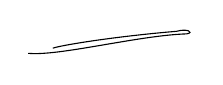
\begin{tikzpicture}[x=0.65cm,y=0.65cm]
\draw[line width=0.4pt] (0,0) .. controls (0.6,-0.06) and (2.15,0.35) .. (3.1,0.38) .. controls (3.25,0.41) and (3.1,0.49) .. (2.9,0.43) .. controls (1.7,0.33) and (0.65,0.16) .. (0.48,0.10);
\end{tikzpicture}}}}
p.24, dernière ligne : dommage qu'on ne do\deleted{t}n\deleted{\unsure{e|a}}ne pas de \deleted{\unsure{m}}démonstration.

p.25, li.8 : ``le soin de'' et non ``de''. Répétition \deleted{\unsure{malsonnante}} de ``développer''.

p.25, li.13 du bas : ``on peut construire $S'$ '' et non ``... $S$''

% archive sheet number: 70
